% Tento soubor nahraďte vlastním souborem s přílohami (nadpisy níže jsou pouze pro příklad)
% This file should be replaced with your file with an appendices (headings below are examples only)

% Umístění obsahu paměťového média do příloh je vhodné konzultovat s vedoucím
% Placing of table of contents of the memory media here should be consulted with a supervisor
%\chapter{Obsah přiloženého paměťového média}

%\chapter{Manuál}

%\chapter{Konfigurační soubor} % Configuration file

%\chapter{RelaxNG Schéma konfiguračního souboru} % Scheme of RelaxNG configuration file

%\chapter{Plakát} % poster

\chapter{Obsah CD}
Na priloženom disku sa nachádza:
\begin{itemize}
\item \textbf{3D modely} -- Jednoduché 3D modely vo formáte OBJ
\item \textbf{Aplikácia} -- V tomto priečinku sa nachádza spustiteľná aplikácia
\item \textbf{Dokumentácia Latex} -- Zdrojový kód dokumentácie v Latex
\item \textbf{Unity projekt} -- Tento priečinok obsahuje Unity projekt zahrňujúci zdrojové súbory
\item \textbf{Videá} -- Videá zobrazujúce vytvorenú aplikáciu
\item \textbf{Bakalárska práca.pdf} -- Dokumentácia k práci
\item \textbf{Plagát.pdf} -- Vytvorený plagát
\item \textbf{Readme.txt} -- Obsahuje informácie o práci
\end{itemize}


\chapter{Ďaľšie vytvorené objekty}

%obrazky dalsich modelov
\begin{figure}[!h]
\centering
\tmpframe{\includegraphics[height=0.32\linewidth]{obrazky-figures/CreatedObjects/Dalsie/IMG_1714.png}}\quad
\tmpframe{\includegraphics[height=0.32\linewidth]{obrazky-figures/CreatedObjects/Dalsie/IMG_1716.png}}\quad
\tmpframe{\includegraphics[height=0.32\linewidth]{obrazky-figures/CreatedObjects/Dalsie/IMG_1720.png}}\quad
\tmpframe{\includegraphics[height=0.32\linewidth]{obrazky-figures/CreatedObjects/Dalsie/IMG_1722.png}}\quad
\tmpframe{\includegraphics[height=0.32\linewidth]{obrazky-figures/CreatedObjects/Dalsie/IMG_1723.png}}\quad
\tmpframe{\includegraphics[height=0.32\linewidth]{obrazky-figures/CreatedObjects/Dalsie/IMG_1725.png}}
\caption{Na obrázkoch je vidieť ďalšie vytvorené objekty. Cubotaherdon, torusy, guľa, octahedron a ihlan.}
\label{fig:dalsie}
\end{figure}


\chapter{Vytvorená skladačka}
Na nasledujúcich stranách je zobrazená skladačka cubotahedronu. Táto skladačka reprezentuje export z vytvoreného programu do formátu PDF s farebným vyplnením plátkov. Pomocou tejto vystrihovačky sa dá poskladať rovnaký objekt ako je vidieť na obrázku \ref{fig:cubotahedron}.
% \todo{Ako to mám dať aby to dobre vyzeralo?}
% %vytvorený 
% \begin{figure}[!h]
% \centering
% \tmpframe{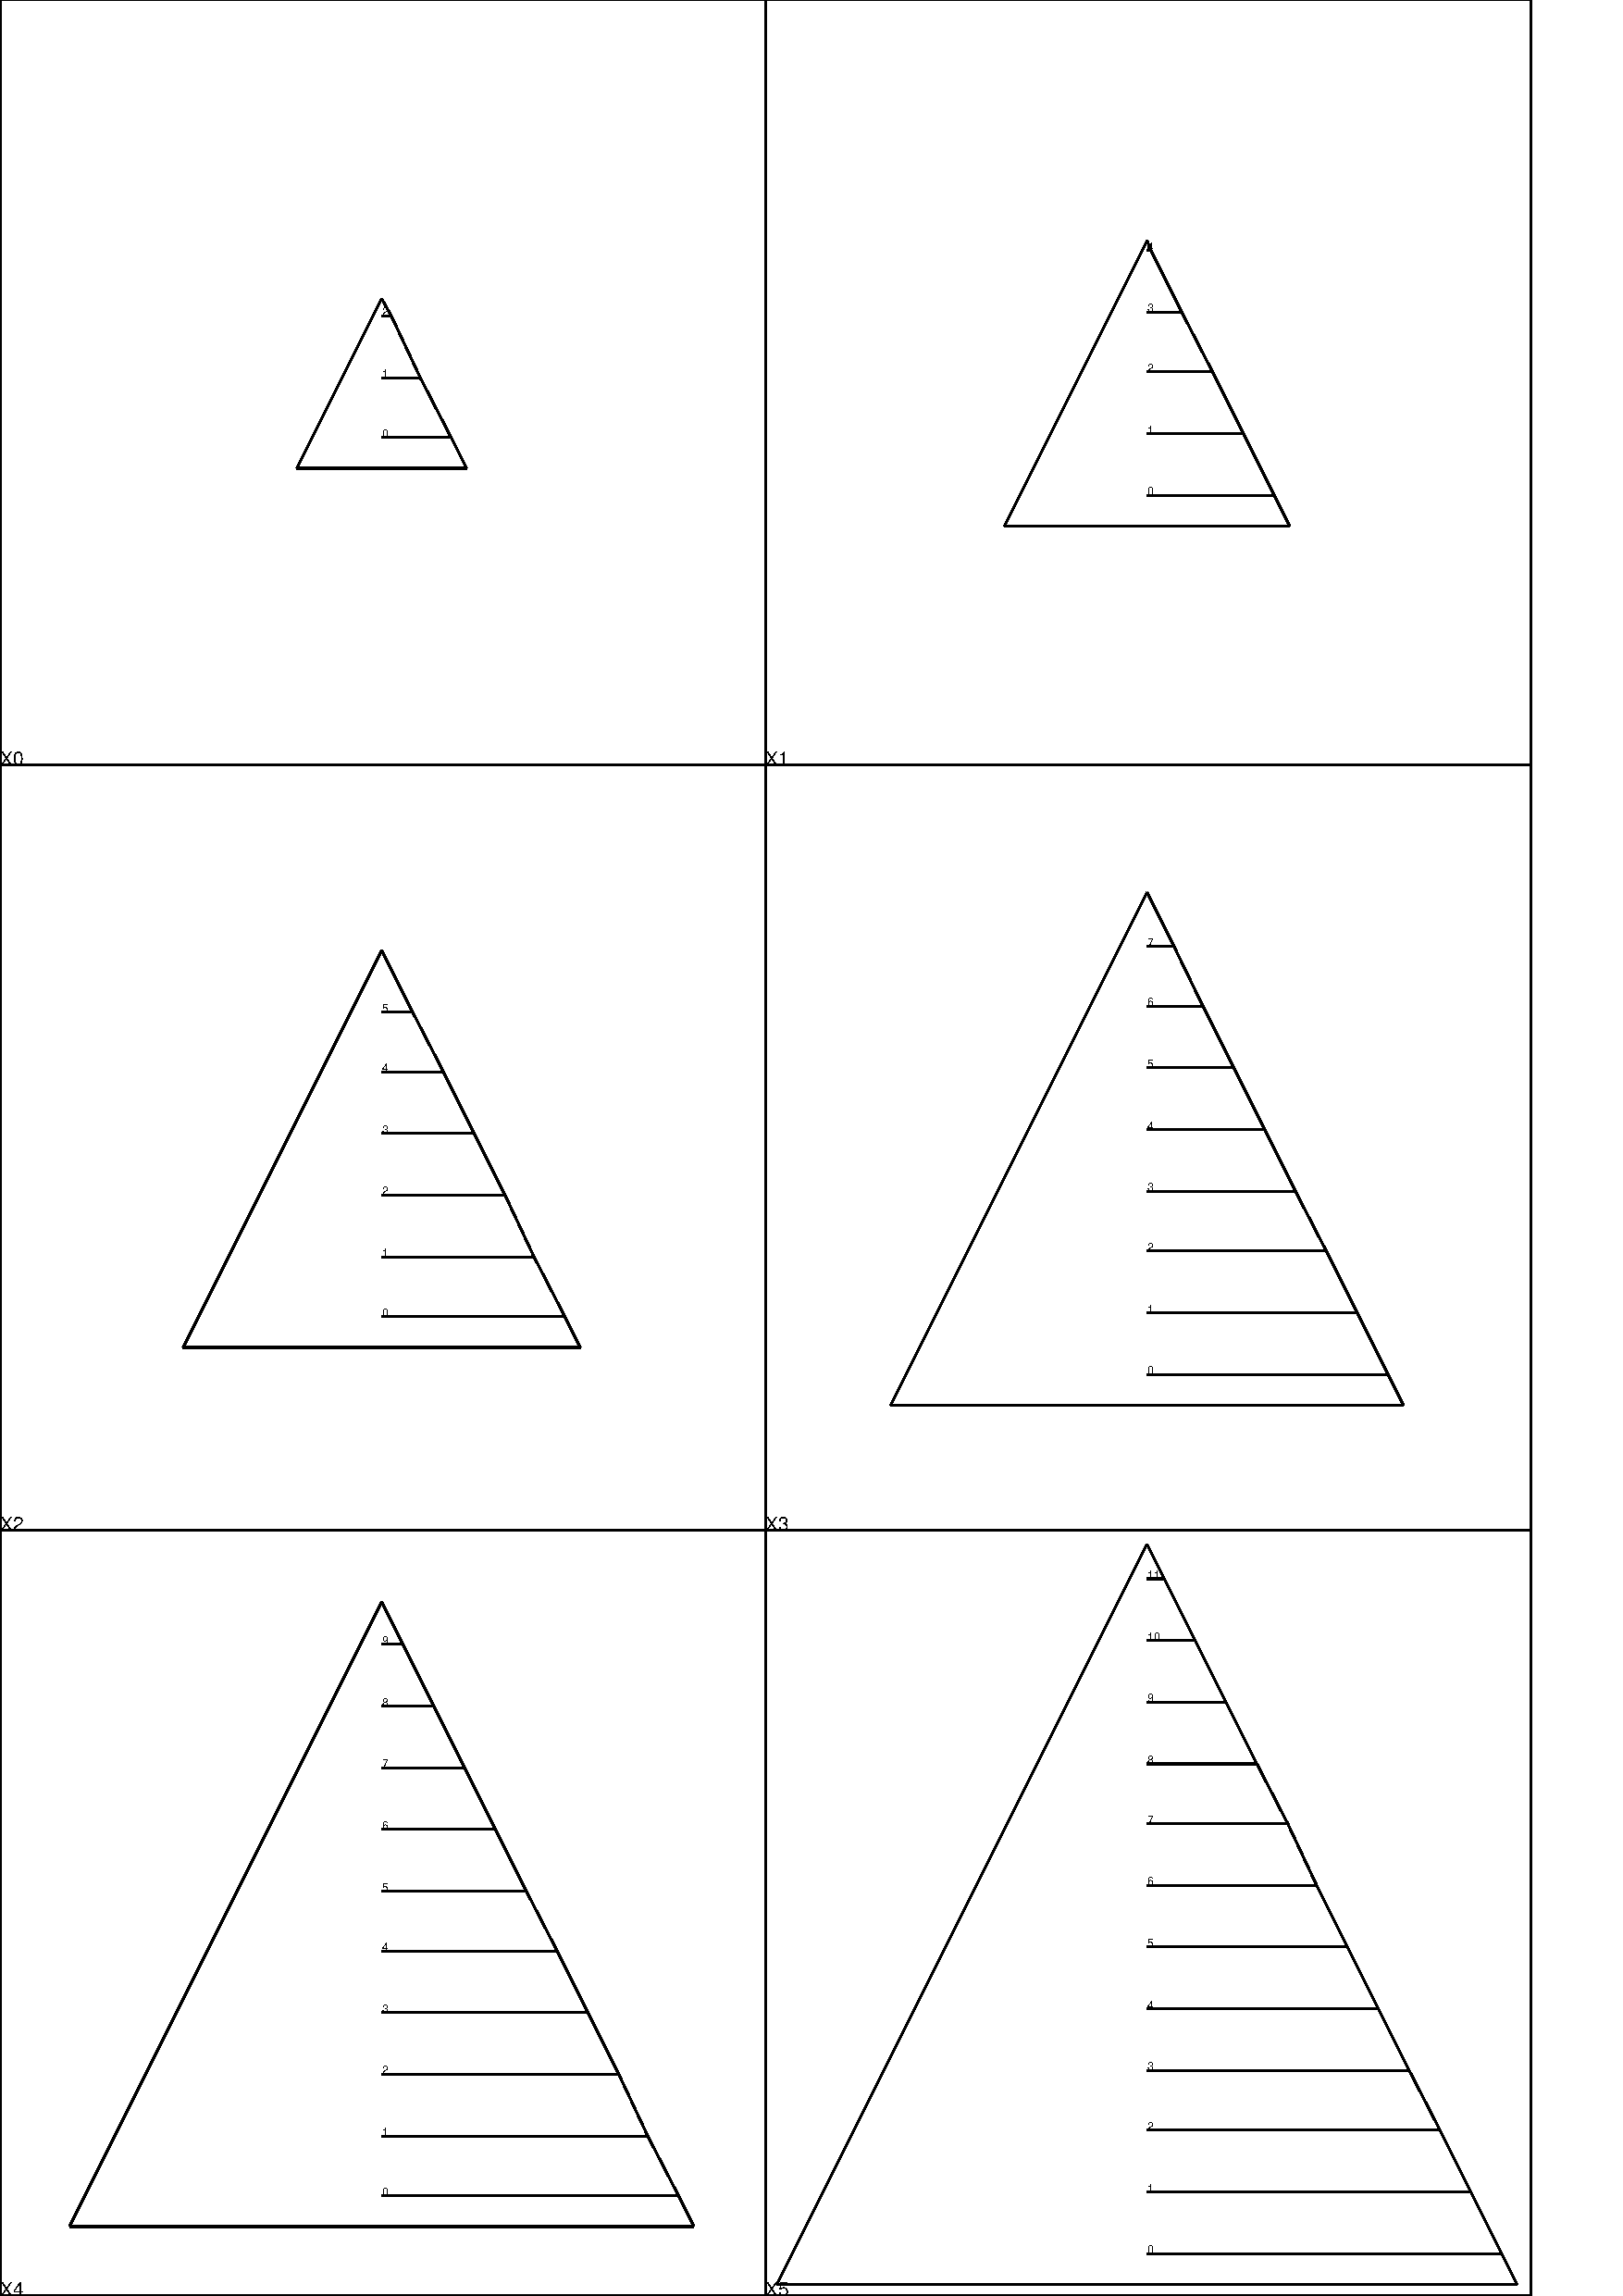
\includegraphics[page=1,height=0.8\linewidth,angle=90,origin=c]{obrazky-figures/ihlan.pdf}}
% \quad
% \tmpframe{\includegraphics[page=2,height=0.8\linewidth,angle=90,origin=c]{obrazky-figures/ihlan.pdf}}
% \caption{X-ové rezy štvorstenného ihlanu}
% \end{figure}
% \begin{figure}[!h]
% \centering
% \tmpframe{\includegraphics[page=3,height=0.8\linewidth,angle=90,origin=c]{obrazky-figures/ihlan.pdf}}
% \quad
% \tmpframe{\includegraphics[page=4,height=0.8\linewidth,angle=90,origin=c]{obrazky-figures/ihlan.pdf}}
% \caption{Y-ové rezy štvorstenného ihlanu}\label{fig:ihlan}
% \end{figure}

\includepdf[pages=1,offset=1.85cm -1.5cm,width=1.2\textwidth]{obrazky-figures/cubotahedron-Sliceforms.pdf}
\includepdf[pages=2,offset=1.85cm -1.5cm,width=1.2\textwidth]{obrazky-figures/cubotahedron-Sliceforms.pdf}
\includepdf[pages=3,offset=1.85cm -1.5cm,width=1.2\textwidth]{obrazky-figures/cubotahedron-Sliceforms.pdf}
\includepdf[pages=4,offset=1.85cm -1.5cm,width=1.2\textwidth]{obrazky-figures/cubotahedron-Sliceforms.pdf}